

\documentclass[DIV=calc, paper=a4, fontsize=13pt, twocolumn]{scrartcl}	 % A4 paper and 11pt font size

\usepackage{lipsum} % Used for inserting dummy 'Lorem ipsum' text into the template
\usepackage[english]{babel} % English language/hyphenation
\usepackage[protrusion=true,expansion=true]{microtype} % Better typography
\usepackage{amsmath,amsfonts,amsthm} % Math packages
\usepackage[svgnames]{xcolor} % Enabling colors by their 'svgnames'
\usepackage[hang, small,labelfont=bf,up,textfont=it,up]{caption} % Custom captions under/above floats in tables or figures
\usepackage{booktabs} % Horizontal rules in tables
\usepackage{fix-cm}	 % Custom font sizes - used for the initial letter in the document

\usepackage{sectsty} % Enables custom section titles
\allsectionsfont{\usefont{OT1}{phv}{b}{n}} % Change the font of all section commands

\usepackage{fancyhdr} % Needed to define custom headers/footers
\pagestyle{fancy} % Enables the custom headers/footers
\usepackage{lastpage} % Used to determine the number of pages in the document (for "Page X of Total")

\usepackage{graphicx}
%\graphicspath{ {Triplex MDH 140 C} }
 
 


% Headers - all currently empty
\lhead{}
\chead{}
\rhead{}

% Footers
\lfoot{}
\cfoot{}
\rfoot{\footnotesize Page \thepage\ of \pageref{LastPage}} % "Page 1 of 2"

\renewcommand{\headrulewidth}{0.0pt} % No header rule
\renewcommand{\footrulewidth}{0.4pt} % Thin footer rule

\usepackage{lettrine} % Package to accentuate the first letter of the text
\newcommand{\initial}[1]{ % Defines the command and style for the first letter
\lettrine[lines=3,lhang=0.3,nindent=0em]{
\color{DarkGoldenrod}
{\textsf{#1}}}{}}

%----------------------------------------------------------------------------------------
%	TITLE SECTION
%----------------------------------------------------------------------------------------

\usepackage{titling} % Allows custom title configuration

\newcommand{\HorRule}{\color{DarkGoldenrod} \rule{\linewidth}{1pt}} % Defines the gold horizontal rule around the title

\pretitle{\vspace{-30pt} \begin{flushleft} \HorRule \fontsize{50}{50} \usefont{OT1}{phv}{b}{n} \color{DarkRed} \selectfont} % Horizontal rule before the title

\title{Abels lifting operations} % Your article title

\posttitle{\par\end{flushleft}\vskip 0.5em} % Whitespace under the title

\preauthor{\begin{flushleft}\large \lineskip 0.5em \usefont{OT1}{phv}{b}{sl} \color{DarkRed}} % Author font configuration

\author{Sebastian Gjertsen, } % Your name

\postauthor{\footnotesize \usefont{OT1}{phv}{m}{sl} \color{DarkBlue} % Configuration for the institution name
University of Oslo % Your institution

\par\end{flushleft}\HorRule} % Horizontal rule after the title

\date{} % Add a date here if you would like one to appear underneath the title block

%----------------------------------------------------------------------------------------

\begin{document}

\maketitle % Print the title

\thispagestyle{fancy} % Enabling the custom headers/footers for the first page 

%----------------------------------------------------------------------------------------
%	ABSTRACT
%----------------------------------------------------------------------------------------

% The first character should be within \initial{}
\initial{A}\textbf{bels lifting operations is a long standing operator in the lifting and installing offshore industry. We have many successful offshore installations over the years. We offer installations in a secure and efficient manner. This appendix will cover the steps involved in installing 16 torpedo anchors. Starting from picking up the anchors onshore to installation on sea floor.}

%----------------------------------------------------------------------------------------
%	ARTICLE CONTENTS
%----------------------------------------------------------------------------------------


%------------------------------------------------
\begin{figure}[h]
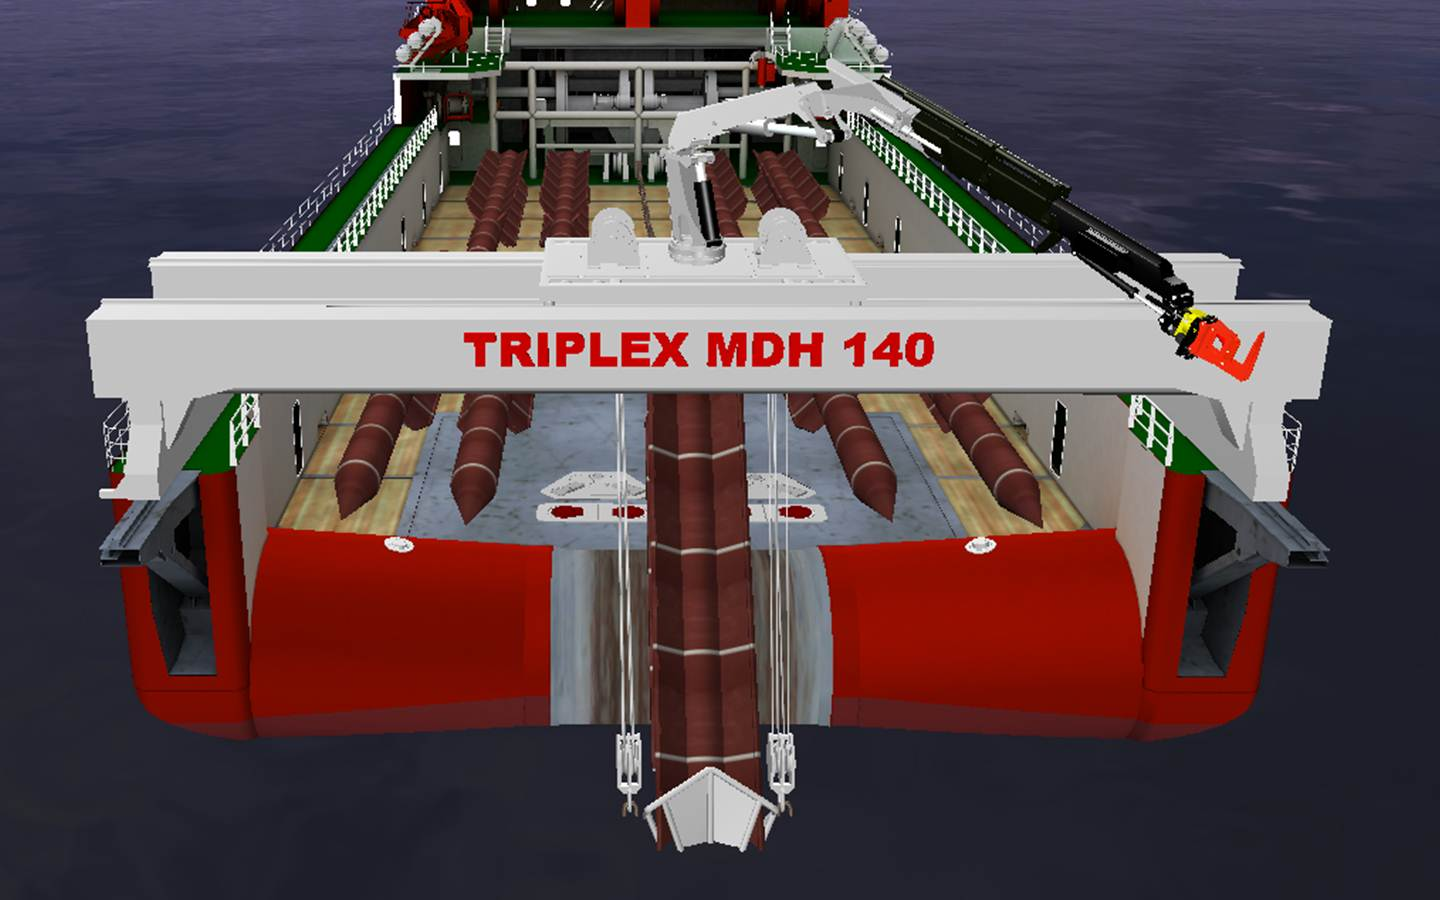
\includegraphics[width=9cm,height=9cm]{Triplex_MDH_140_C.jpg}
\end{figure}

\subsection*{Onshore and Load out}
In this operation we need only a crane vessel, which will also serve as a transportation vessel. By only using one vessel we will save money and time. But it will need to be carefully planned in regards to deck space and lift out. The vessel we recommend is the Triplex MDH 140. Specs
\begin{itemize}
\item Handles anchors of 120 tons
\item Large deck space that can take all 16 anchors 
\item Launches a torpedo from anywhere on deck in 5 minutes
\item Handles rough weather
\end{itemize}
The crane will be used to load the torpedoes side by side parallel to the direction of travel. We will get 10 of the torpedoes on the floor of the deck. The additional 6 will be stacked with 3 on each side on top of the others. Leaving the middle with only one in height. This arrangement is done so to have a easy load out period. Where we start from the middle anchor and work our way out. 
\newline
The second part of the operation will be to practice the lift out from the vessel into the water. As this is a crucial part of the operation where many errors can occur. When we lift an anchor weighing 50 tons from the floor of a vessel and horizontally out to sea, the shift in the vessels balance may seriously be compromised. This fact and the dynamic forces of the waves and weather, will make this a delicate procedure. It is also good to check that the winch works as intended. 
\newline
I therefore strongly recommend that a short amount of time is used on a practice lift while the vessel is key-side. This will help us in knowing what to expect when we get out to sea. This could in worst case prevent loss of lives and or precious equipment.



\subsection*{Transportation}
The vessel we are using for transportation has been carefully calculated to withstand the force of 800 tons of steel. The vessel will also be searched for cracks and other damages, to ensure the safety of crew and gear. The torpedoes will be layed down side by side and strapped to the deck. Since they are laying down on the deck, the vessel will more or less stable and can endure quite a bit of weather. But when we are to lift out and drop the torpedoes the vessel will be more unstable and a maximum wind profile cannot be overdone. We will use a weather simulating program, and a worst case scenario will be evaluated. We therefore need to plan in accordance with the weather forecasts when the operation will take place. 
\subsection*{Lifting from deck}
\begin{figure}[h]
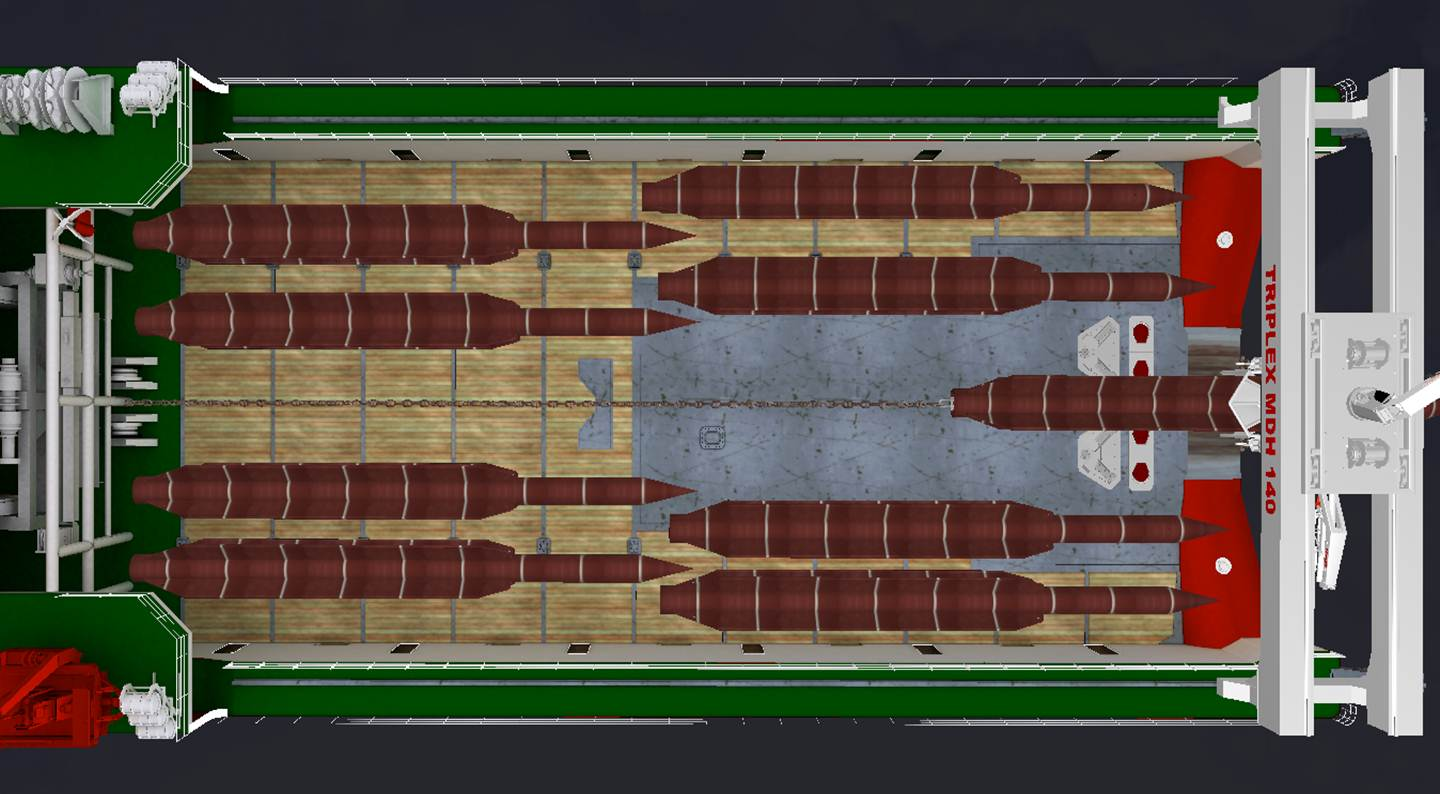
\includegraphics[width=9cm,height=9cm]{Triplex_MDH_140.jpg}
\end{figure}
Since we practiced this part at key side. We have hopefully gained some knowledge and skill. As we see in the picture the torpedoes are laying side by side with front and back facing forward and aft. The crane will pick them up starting in the middle and working outward. The boat is put in position (by GPS) and the torpedoes are hooked up to the winch in the front part of the deck. The crane pulls the torpedo all the way back, and then the winch lets the torpedoes slide out the back. At this point where the torpedoes are in the water, we can only tolerate so much weather. Because the stresses on the wires that holds the torpedoes will become big if the boat starts moving too much. Since the torpedoes have to move the surrounding water. In our case the water depth is not that high and we will drop the torpedoes not far under water surface. So resonance in the wire will not be much of a problem. 
\subsection*{Splash and drop}

We now enter a critical face of the operation. When we introduce objects to the water we experience hydrodynamical effects. We will use a time domain analysis, to calculate the worst case effects. These effects will be determined mostly by the frequency and amplitude of the waves. In this operation we have a vessel with a very nice mechanism to deliver the torpedoes to the water. This means that we can handle some weather. Meaning we can save time and money by not having to wait for the perfect weather conditions.
The winches will lower the torpedoes slowly into the water, as they will experience some buoyancy effects, so lowering slowly will assure a tight wire. A slow lowering will also ensure that all the trapped air inside the object will be filled with water and nothing broken. This is not a big deal since we are dealing with an all steel object. Since we will drop the torpedoes topside we will not have problems with the weight of the wire it self causing stress on the system. 
This vessel allows us to deliver the torpedoes with the 'pointy end' down in the water. With the construction of the torpedoes this will ensure us that they hit the sea floor in the same fashion, and gets buried deep for a secure anchor fastening.
\newline 
Usually when installing something on the sea floor we want a smooth landing. But in our case we want just the opposite. The torpedoes will be dropped from topside to unsure a target velocity on the sea bed of $50 \frac{m}{s}$
When released 300 m from the ocean floor the torpedo will reach terminal velocity:
\begin{align}
F &= ma = -mg + \frac{1}{2} \rho C_D v^2 S \\
&\text{The acceleration is zero} \\
&\text{when we reach terminal velocity} \\
v &= \sqrt{\frac{2 * 50 000 kg * 9.81 \frac{m}{s^2}}{1000\frac{kg}{m^3} * 0.2 * 1.5 m^2}} \\
v &= 57.2 \frac{m}{s}
\end{align}
Since we want to drop the anchor as accurate as possible, and need only reach a speed of $50 m/s$. We should lower the anchor so the height above the sea floor is just enough to reach this speed. If we drop the anchors from topside they may drift off their intended landing position. 
\newline
\begin{figure}[t]
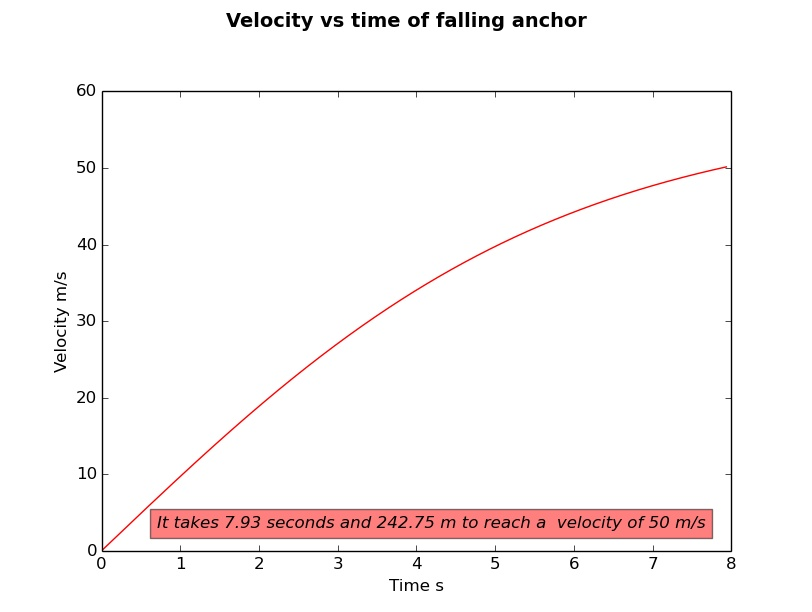
\includegraphics[width=10cm,height=10cm]{velocity_plot.jpg}
\end{figure}
To calculate how far above the sea floor we need to be, to reach a speed of $50 m/s $, I have made a short program that plots the velocity and calculates, using the Trapezoidal method, how far above the sea floor we need to be. 











\begin{description}
\item[First] This is the first item
\item[Last] This is the last item
\end{description}


%----------------------------------------------------------------------------------------
%	REFERENCE LIST
%----------------------------------------------------------------------------------------

\begin{thebibliography}{99} % Bibliography - this is intentionally simple in this template


\newblock http://www.triplex.no/site/view/mdh\_140\_ahts
 
\end{thebibliography}


%----------------------------------------------------------------------------------------

\end{document}